\documentclass{standalone}
\usepackage{tikz}
\usepackage{ctex,siunitx}
\setCJKmainfont{Noto Serif CJK SC}
\usepackage{tkz-euclide}
\usepackage{amsmath}
\usetikzlibrary{patterns, calc,3d}
\usetikzlibrary {decorations.pathmorphing,decorations.pathreplacing,decorations.shapes,}
\tikzset{label style/.append style={font=\small}}
\begin{document}
\small
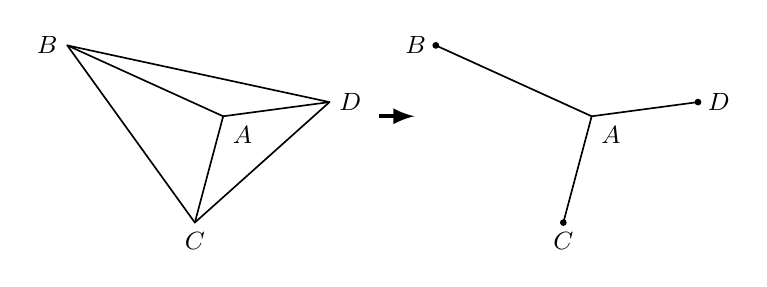
\begin{tikzpicture}[>=latex,scale=0.9]
\begin{scope}
  \tkzDefPoints{0/0/A,-2.2/1.0/B,-0.4/-1.5/C,1.5/0.2/D}
  \tkzDrawPolygon[semithick](B,C,D)
  \tkzDrawSegments[semithick](A,C A,D A,B)
  \tkzLabelPoints(C)
  \tkzLabelPoints[below right](A)
  \tkzLabelPoints[left](B)
  \tkzLabelPoints[right](D)
\end{scope}
\draw[ultra thick,->](2.2,0)--++(0.5,0);
\begin{scope}[xshift=5.2cm]
  \tkzDefPoints{0/0/A,-2.2/1.0/B,-0.4/-1.5/C,1.5/0.2/D}
  \tkzDrawSegments[semithick](A,C A,D A,B)
  \tkzDrawPoints[fill=black](B,C,D)
  \tkzLabelPoints(C)
  \tkzLabelPoints[below right](A)
  \tkzLabelPoints[left](B)
  \tkzLabelPoints[right](D)
\end{scope}
\end{tikzpicture}
\end{document}